\chapter{Architektury přístupových systémů}
\DIFdelbegin %DIFDELCMD < 

%DIFDELCMD < %%%
\DIFdelend Přístupové systémy jsou elektronické systémy řídící přístup uživatelů do omezených prostor v závislosti na jejich prokázané identitě.
Obrázek \ref{fig:Access control system architecture} zobrazuje typickou architekturu přístupového systému, kde \DIFdelbegin \DIFdel{ID Credential }\DIFdelend \DIFaddbegin \DIFadd{identifikátor (ID Credential) }\DIFaddend představuje prvek umožňující identifikovat uživatele, např. RFID tag, otisk prstu nebo QR kód. 

\begin{figure}[!h]
    \centering
    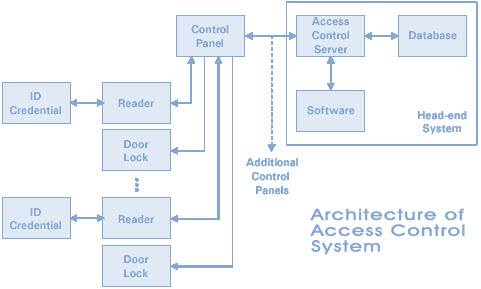
\includegraphics[width=130mm]{Architetcture-of-Access-Control-System}
    \caption{Příklad architektury přístupového systému \cite{accessControlSystem_eiprocus}}
    \label{fig:Access control system architecture}
\end{figure}

\DIFdelbegin \DIFdel{Zařízení typu Reader}\DIFdelend \DIFaddbegin \DIFadd{Čtečka (Reader) }\DIFaddend slouží ke čtení dat z \DIFdelbegin \DIFdel{ID Credential }\DIFdelend \DIFaddbegin \DIFadd{identifikátoru }\DIFaddend a v digitální podobě je odesílá k zařízení \DIFdelbegin \DIFdel{typu Control Panel.
Zařízení typu Door Lock}\DIFdelend \DIFaddbegin \DIFadd{kontrolní panel (Control Panel).
Zámek dveří (Door Lock) }\DIFaddend řídí fyzický přístup uživatelů do omezených prostor. 
\DIFdelbegin \DIFdel{Zařízení typu Control Panel }\DIFdelend \DIFaddbegin \DIFadd{Kontrolní panel }\DIFaddend tvoří rozhranní mezi Access Control Server a páry \DIFdelbegin \DIFdel{zařízení typů Reader a Door Lock.
Zařízení typu Control Panel jsou obvykle připojena 
k zařízení typu }\DIFdelend \DIFaddbegin \DIFadd{čteček a zámků dveří.
kontrolní panely jsou obvykle připojeny k serveru řízení přístupu (}\DIFaddend Access Control Server\DIFaddbegin \DIFadd{) }\DIFaddend přes TCP/IP síť a páry \DIFdelbegin \DIFdel{zařízení typů Reader a Door Lock }\DIFdelend \DIFaddbegin \DIFadd{čtečka a zámků dveří }\DIFaddend jsou obvykle připojeny \DIFdelbegin \DIFdel{k zařízení typu Control panel }\DIFdelend \DIFaddbegin \DIFadd{ke kontrolnímu panelu }\DIFaddend přes RS485 síť. Databáze obsahuje všechna uživatelské ID.
Na \DIFdelbegin \DIFdel{Access Control Serveru }\DIFdelend \DIFaddbegin \DIFadd{serveru řízení přístupu }\DIFaddend je spuštěn Software (SW) spravující databázi a komunikující se všemi zařízeními typu Contril Panel.
\DIFdelbegin \DIFdel{Zařízení typu Reader }\DIFdelend \DIFaddbegin \DIFadd{Čtečka }\DIFaddend čte uživatelská ID z předložených \DIFdelbegin \DIFdel{ID Credential }\DIFdelend \DIFaddbegin \DIFadd{identifikátorů }\DIFaddend a přeposílá je \DIFdelbegin \DIFdel{k zařízení typu Control Panel, které }\DIFdelend \DIFaddbegin \DIFadd{na kontrolní panel, který }\DIFaddend je dále přeposílá na \DIFdelbegin \DIFdel{Access Control Server}\DIFdelend \DIFaddbegin \DIFadd{server řízení přístupu}\DIFaddend . 
Access Control Software vyhledá \DIFdelbegin \DIFdel{obdržená uživatelská ID }\DIFdelend \DIFaddbegin \DIFadd{obdržený uživatelský identifikátor }\DIFaddend v databázi a pokud je \DIFdelbegin \DIFdel{nalezeno}\DIFdelend \DIFaddbegin \DIFadd{nalezen}\DIFaddend , pošle příkaz odpovídajícímu \DIFdelbegin \DIFdel{zařízení typu Control Panel }\DIFdelend \DIFaddbegin \DIFadd{kontrolnímu panelu }\DIFaddend k přepnutí odpovídajícímu \DIFdelbegin \DIFdel{zařízení typu Door Lock}\DIFdelend \DIFaddbegin \DIFadd{zámku dveří}\DIFaddend , čímž je uživateli udělen přístup do omezené oblasti \cite{accessControlSystem_eiprocus}.
